%-----------------------------------------------------------------------------------------------------------------------------------------------%
%	The MIT License (MIT)
%
%	Copyright (c) 2021 Jitin Nair
%
%	Permission is hereby granted, free of charge, to any person obtaining a copy
%	of this software and associated documentation files (the "Software"), to deal
%	in the Software without restriction, including without limitation the rights
%	to use, copy, modify, merge, publish, distribute, sublicense, and/or sell
%	copies of the Software, and to permit persons to whom the Software is
%	furnished to do so, subject to the following conditions:
%	
%	THE SOFTWARE IS PROVIDED "AS IS", WITHOUT WARRANTY OF ANY KIND, EXPRESS OR
%	IMPLIED, INCLUDING BUT NOT LIMITED TO THE WARRANTIES OF MERCHANTABILITY,
%	FITNESS FOR A PARTICULAR PURPOSE AND NONINFRINGEMENT. IN NO EVENT SHALL THE
%	AUTHORS OR COPYRIGHT HOLDERS BE LIABLE FOR ANY CLAIM, DAMAGES OR OTHER
%	LIABILITY, WHETHER IN AN ACTION OF CONTRACT, TORT OR OTHERWISE, ARISING FROM,
%	OUT OF OR IN CONNECTION WITH THE SOFTWARE OR THE USE OR OTHER DEALINGS IN
%	THE SOFTWARE.
%	
%
%-----------------------------------------------------------------------------------------------------------------------------------------------%

%----------------------------------------------------------------------------------------
%	DOCUMENT DEFINITION
%----------------------------------------------------------------------------------------

% article class because we want to fully customize the page and not use a cv template
\documentclass[a4paper,12pt]{article}

%----------------------------------------------------------------------------------------
%	FONT
%----------------------------------------------------------------------------------------

% % fontspec allows you to use TTF/OTF fonts directly
% \usepackage{fontspec}
% \defaultfontfeatures{Ligatures=TeX}

% % modified for ShareLaTeX use
% \setmainfont[
% SmallCapsFont = Fontin-SmallCaps.otf,
% BoldFont = Fontin-Bold.otf,
% ItalicFont = Fontin-Italic.otf
% ]
% {Fontin.otf}

%----------------------------------------------------------------------------------------
%	PACKAGES
%----------------------------------------------------------------------------------------
\usepackage{url}
\usepackage{parskip} 	
\usepackage{soul}

%other packages for formatting
\RequirePackage{color}
\RequirePackage{graphicx}
\usepackage[usenames,dvipsnames]{xcolor}
\usepackage[scale=0.9]{geometry}

%tabularx environment
\usepackage{tabularx}

%for lists within experience section
\usepackage{enumitem}

% centered version of 'X' col. type
\newcolumntype{C}{>{\centering\arraybackslash}X} 

%to prevent spillover of tabular into next pages
\usepackage{supertabular}
\usepackage{tabularx}
\newlength{\fullcollw}
\setlength{\fullcollw}{0.47\textwidth}

%custom \section
\usepackage{titlesec}				
\usepackage{multicol}
\usepackage{multirow}

%CV Sections inspired by: 
%http://stefano.italians.nl/archives/26
\titleformat{\section}{\Large\scshape\raggedright}{}{0em}{}[\titlerule]
\titlespacing{\section}{0pt}{10pt}{10pt}

%for publications
\usepackage[style=numeric,sorting=ydnt, maxbibnames=99]{biblatex}

%Setup hyperref package, and colours for links
\usepackage[unicode, draft=false]{hyperref}
\definecolor{linkcolour}{HTML}{BF0707}
\hypersetup{colorlinks,breaklinks,urlcolor=linkcolour,linkcolor=linkcolour, colorlinks=true}

\addbibresource{citations.bib}
\setlength\bibitemsep{1em}

%for social icons
\usepackage{fontawesome5}

%debug page outer frames
%\usepackage{showframe}


% job listing environments
\newenvironment{jobshort}[2]
    {
    \begin{tabularx}{\linewidth}{@{}l X r@{}}
    \textbf{#1} & \hfill &  #2 \\[3.75pt]
    \end{tabularx}
    }
    {
    }

\newenvironment{joblong}[2]
    {
    \begin{tabularx}{\linewidth}{@{}l X r@{}}
    \textbf{#1} & \hfill &  #2 \\[3.75pt]
    \end{tabularx}
    \begin{minipage}[t]{\linewidth}
    \begin{itemize}[nosep,after=\strut, leftmargin=1em, itemsep=3pt,label=--]
    }
    {
    \end{itemize}
    \end{minipage}    
    }


\renewcommand{\arraystretch}{1.5}
%----------------------------------------------------------------------------------------
%	BEGIN DOCUMENT
%----------------------------------------------------------------------------------------
\begin{document}

% non-numbered pages
\pagestyle{empty} 

%----------------------------------------------------------------------------------------
%	TITLE
%----------------------------------------------------------------------------------------

% \begin{tabularx}{\linewidth}{ @{}X X@{} }
% \huge{Your Name}\vspace{2pt} & \hfill \emoji{incoming-envelope} email@email.com \\
% \raisebox{-0.05\height}\faGithub\ username \ | \
% \raisebox{-0.00\height}\faLinkedin\ username \ | \ \raisebox{-0.05\height}\faGlobe \ mysite.com  & \hfill \emoji{calling} number
% \end{tabularx}

\begin{tabularx}{\linewidth}{@{}l@{} l @{}}
\multirow{2}{4cm}{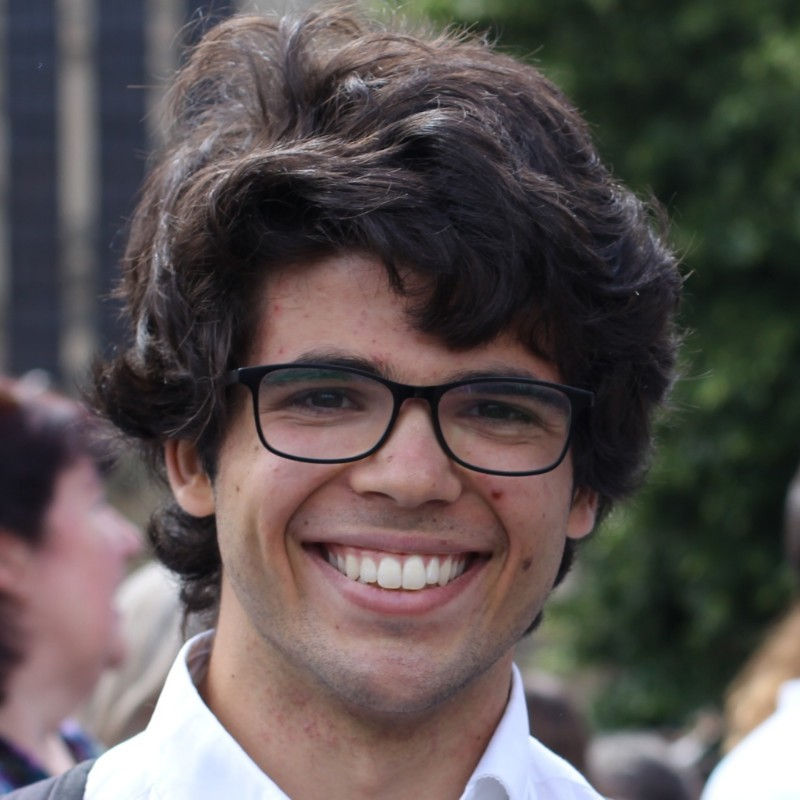
\includegraphics[width=0.2\textwidth]{pic.jpeg}}&\\
&\\
&\Huge{Gabriele Benedetti}\\
& \today \ $|$ \ \href{https://github.com/gbene}{https://github.com/gbene} \ $|$\\
& \href{https://gabri.xyz}{https://gabri.xyz} \ $|$ \ \href{mailto:mail@gabri.xyz}{mail@gabri.xyz} \\
\end{tabularx}

% \vspace{2cm}
%----------------------------------------------------------------------------------------
% EXPERIENCE SECTIONS
%----------------------------------------------------------------------------------------

%Experience
\section{Work Experience}

\begin{jobshort}{University research assistant}{Feb 2023 - Aug 2025}
    \textit{University of Milano-Bicocca | Milano, Italy}
    \begin{itemize}
        \item Point cloud segmentation procedures for fracture planes extraction
        \item Right censoring bias estimation and correction for fracture length statistical modelling
        \item Stochastic DFN parameter calibration
    \end{itemize}
\end{jobshort}


\begin{jobshort}{Programmer}{May 2022 - Feb 2023}
    \textit{Pro Iter Ambiente s.r.l. | Milano, Italy}
    \newline
    Development of the PZero software
    \begin{itemize}
        \item User interface and quality of life improvements
        \item Backend refactorization
        \item Wells and geophyisical profiles integration 
        \item Streamline input and output with CAD/BIM environments 
    \end{itemize}
\end{jobshort}


\begin{jobshort}{Programmer}{Nov 2019 - Dic 2019}
    \textit{Freelance | Milano, Italy}

    Designed and programmed an Agisoft Metashape compatilbe pipeline to calculate the elevation difference between two models. 
\end{jobshort}

%----------------------------------------------------------------------------------------
%	EDUCATION
%----------------------------------------------------------------------------------------
\section{Education}
\begin{tabularx}{\linewidth}{@{}l X@{} @{}r}	
2025 - present & PhD in Geophysics\newline \textit{\underline{University of Iceland} | Reykavik, Iceland}& \\

2020 - 2022 & \textbf{MSc in Geology and Geodynamis} \newline \textit{\underline{University of Milano-Bicocca} | Milano, Italy} & (110/110 cum laude)\\
\textbf{Thesis} & \multicolumn{2}{l}{New tools for Digital Outcrop Models analysis: Implementation for
the PZero software} \\
\textbf{Keywords} & \multicolumn{2}{p{0.8\textwidth}}{Structural geology data analysis, Full stack development, Principal Component Analysis, Automatic segmentation, Clustering algorithm, VTK}\\

2017-2020 & \textbf{BSc in Geological and Geotechnical sciences} \newline \textit{\underline{University of Milano-Bicocca} | Milano, Italy} & (107/110)\\
\textbf{Thesis} & \multicolumn{2}{l}{Photogrammetric techniques applied to invertebrate paleontology} \\
\textbf{Keywords} & \multicolumn{2}{p{0.8\textwidth}}{Photogrammetry, Agisoft Metashape, Preservation and archival}\\

% \newline 
% \newline 
% \begin{itemize}
%     \item \textbf{Thesis}: New tools for Digital Outcrop Models analysis: Implementation for the PZero software
%     \item \textbf{Key arguments}: Structural geology data analysis, Full stack development, Principal Component Analysis, Automatic segmentation, Clustering algorithm, VTK
% \end{itemize} \\ 

% 2017-2020 & \textbf{BSc in Geological science and Geotechnics} \hfill  (107/110) 
% \newline \textit{\underline{University of Milano-Bicocca} | Milano, Italy}
% \newline
% \begin{itemize}
%     \item \textbf{Thesis}: Photogrammetric techniques applied to invertebrate paleontology
%     \item \textbf{Key arguments}: Photogrammetry, Agisoft Metashape, Preservation and archival
% \end{itemize} \\ 

\end{tabularx}
\newpage

%----------------------------------------------------------------------------------------
%	PUBLICATIONS
%----------------------------------------------------------------------------------------
\section{Publications}
\begin{refsection}[citations.bib]
\nocite{*}
\printbibliography[heading=none]
\end{refsection}

\section{Conferences and Awards}
\begin{tabularx}{\linewidth}{@{}l X r}	

2025 & \textbf{European Geosciences Union} [\href{https://meetingorganizer.copernicus.org/EGU25/EGU25-13050.html}{link}] & (\textit{Wien, Austria})\\
& \multicolumn{2}{l}{Asperity cycle simulation using observed seismicity: Applications to the Bardarbunga caldera}\\

2024 & \textbf{Deformation Mechanisms, Rheology and Tectonics} & (\textit{\underline{Best student presentation award}} | \textit{Barcelona, Spain})\\
& \multicolumn{2}{p{0.8\textwidth}}{Scale independent unbiased statistical length analysis of linear features: Adapting survival analysis techniques to geological applications}\\

2024 & \textbf{European Geosciences Union} [\href{https://meetingorganizer.copernicus.org/EGU24/EGU24-22156.html}{link}] & (\textit{\underline{OSPP award}} | \textit{Wien, Austria})\\

& \multicolumn{2}{l}{FracAbility: A python toolbox for survival analysis in fractured rock systems}\\

2024 & \textbf{Tectonic Studies Group} & (\textit{St. Andrews, UK})\\

& \multicolumn{2}{l}{FracAbility: A python toolbox for survival analysis in fractured rock systems}\\

2023 & \textbf{Congresso congiunto SIMP, SGI, SOGEI, AIV} & (\textit{Potenza, Italy})\\

& \multicolumn{2}{l}{Methods for merging fragmented facets obtained from point cloud segmentation algorithms.}\\

2023 & \textbf{European Geosciences Union} [\href{https://meetingorganizer.copernicus.org/EGU23/EGU23-9549.html}{link}] & (\textit{Wien, Austria})\\

& \multicolumn{2}{l}{Point cloud analysis and segmentation procedures in the PZero software}\\

\end{tabularx}

%----------------------------------------------------------------------------------------
%	PROJECTS
%----------------------------------------------------------------------------------------
\section{Projects}

\begin{itemize}

    \item \href{https://github.com/gbene/HighSeas.jl}{HighSeas.jl} | SEAS simulations with High Performance Computing in mind 
    \item \href{https://github.com/gbene/Squiggles.jl}{Squiggles.jl} | Julia package to accelerate 1D cross correlations of seismic signals using any GPU
    \item \href{https://github.com/gecos-lab/FracAbility}{Fracability} | Python toolbox to analyse fracture networks for digitalized rock outcrops 
    \item \href{https://github.com/gbene/Fractalizer.jl}{Fractalizer.jl} | Fractalize any shape
    \item \href{https://github.com/gbene/SirGridsAlot}{SirGridsAlot} | Lighting fast tilable regular grids in python 
\end{itemize}
% \begin{tabularx}{\linewidth}{ @{}l r@{} }
% \textbf{Some Project} & \hfill \href{https://some-link.com}{Link to Demo} \\[3.75pt]
% \multicolumn{2}{@{}X@{}}{long long line of blah blah that will wrap when the table fills the column width long long line of blah blah that will wrap when the table fills the column width long long line of blah blah that will wrap when the table fills the column width long long line of blah blah that will wrap when the table fills the column width}  \\
% \end{tabularx}


%----------------------------------------------------------------------------------------
%	SKILLS
%----------------------------------------------------------------------------------------
\section{Skills}
\begin{tabularx}{\linewidth}{@{}l X@{}}
\textbf{Languages} & Italian (Native), English (Fluent)\\
\textbf{Programming languages}  &  Python, Julia, CUDA, MATLAB, Bash, CSS/HTML\\
\textbf{Libraries} & numpy, pandas/geopandas, shapely, VTK/pyvista, Makie.jl, CUDA.jl, DiffEq.jl\\
\textbf{Software} & Arc/QGIS, Agisoft Metashape, PZero/SKUA/Petrel/Move, Blender, FreeCAD/KiCAD\\
\textbf{Technologies} & Git, \LaTeX, Markdown, SLURM, Docker, ssh\\
\end{tabularx}
\end{document}
